
%(BEGIN_QUESTION)
% Copyright 2014, Tony R. Kuphaldt, released under the Creative Commons Attribution License (v 1.0)
% This means you may do almost anything with this work of mine, so long as you give me proper credit

Use the ``impedance triangle'' to calculate the impedance of this series combination of resistance ($R$) and inductive reactance ($X$):

$$\includegraphics[width=15.5cm]{i01030x01.eps}$$

Explain what equation(s) you use to calculate $Z$.

\underbar{file i01030}
%(END_QUESTION)





%(BEGIN_ANSWER)

$Z$ = 625 $\Omega$, as calculated by the Pythagorean Theorem.

%(END_ANSWER)





%(BEGIN_NOTES)

Be sure to have students show you the form of the Pythagorean Theorem, rather than showing them yourself, since it is so easy for students to research on their own.

%INDEX% Electronics review: AC reactance and impedance

%(END_NOTES)


